\subsubsection{Hub Reorganization and Subsector-Level Dependencies}
\label{sec:subsector_network}

The changes observed in MST and PMFG topology are also reflected in the identity of the most central assets. Figure~\ref{fig:hub_rank} compares hub rankings before and after removal of the dominant market mode. In the original PMFG, BBDC4 has the highest degree and GGBR4 the highest betweenness, whereas GUAR3 becomes the leading node according to both measures in the group-mode network. The change indicates that centrality depends strongly on whether broad market co-movement is retained in the underlying correlation structure.

\begin{center}
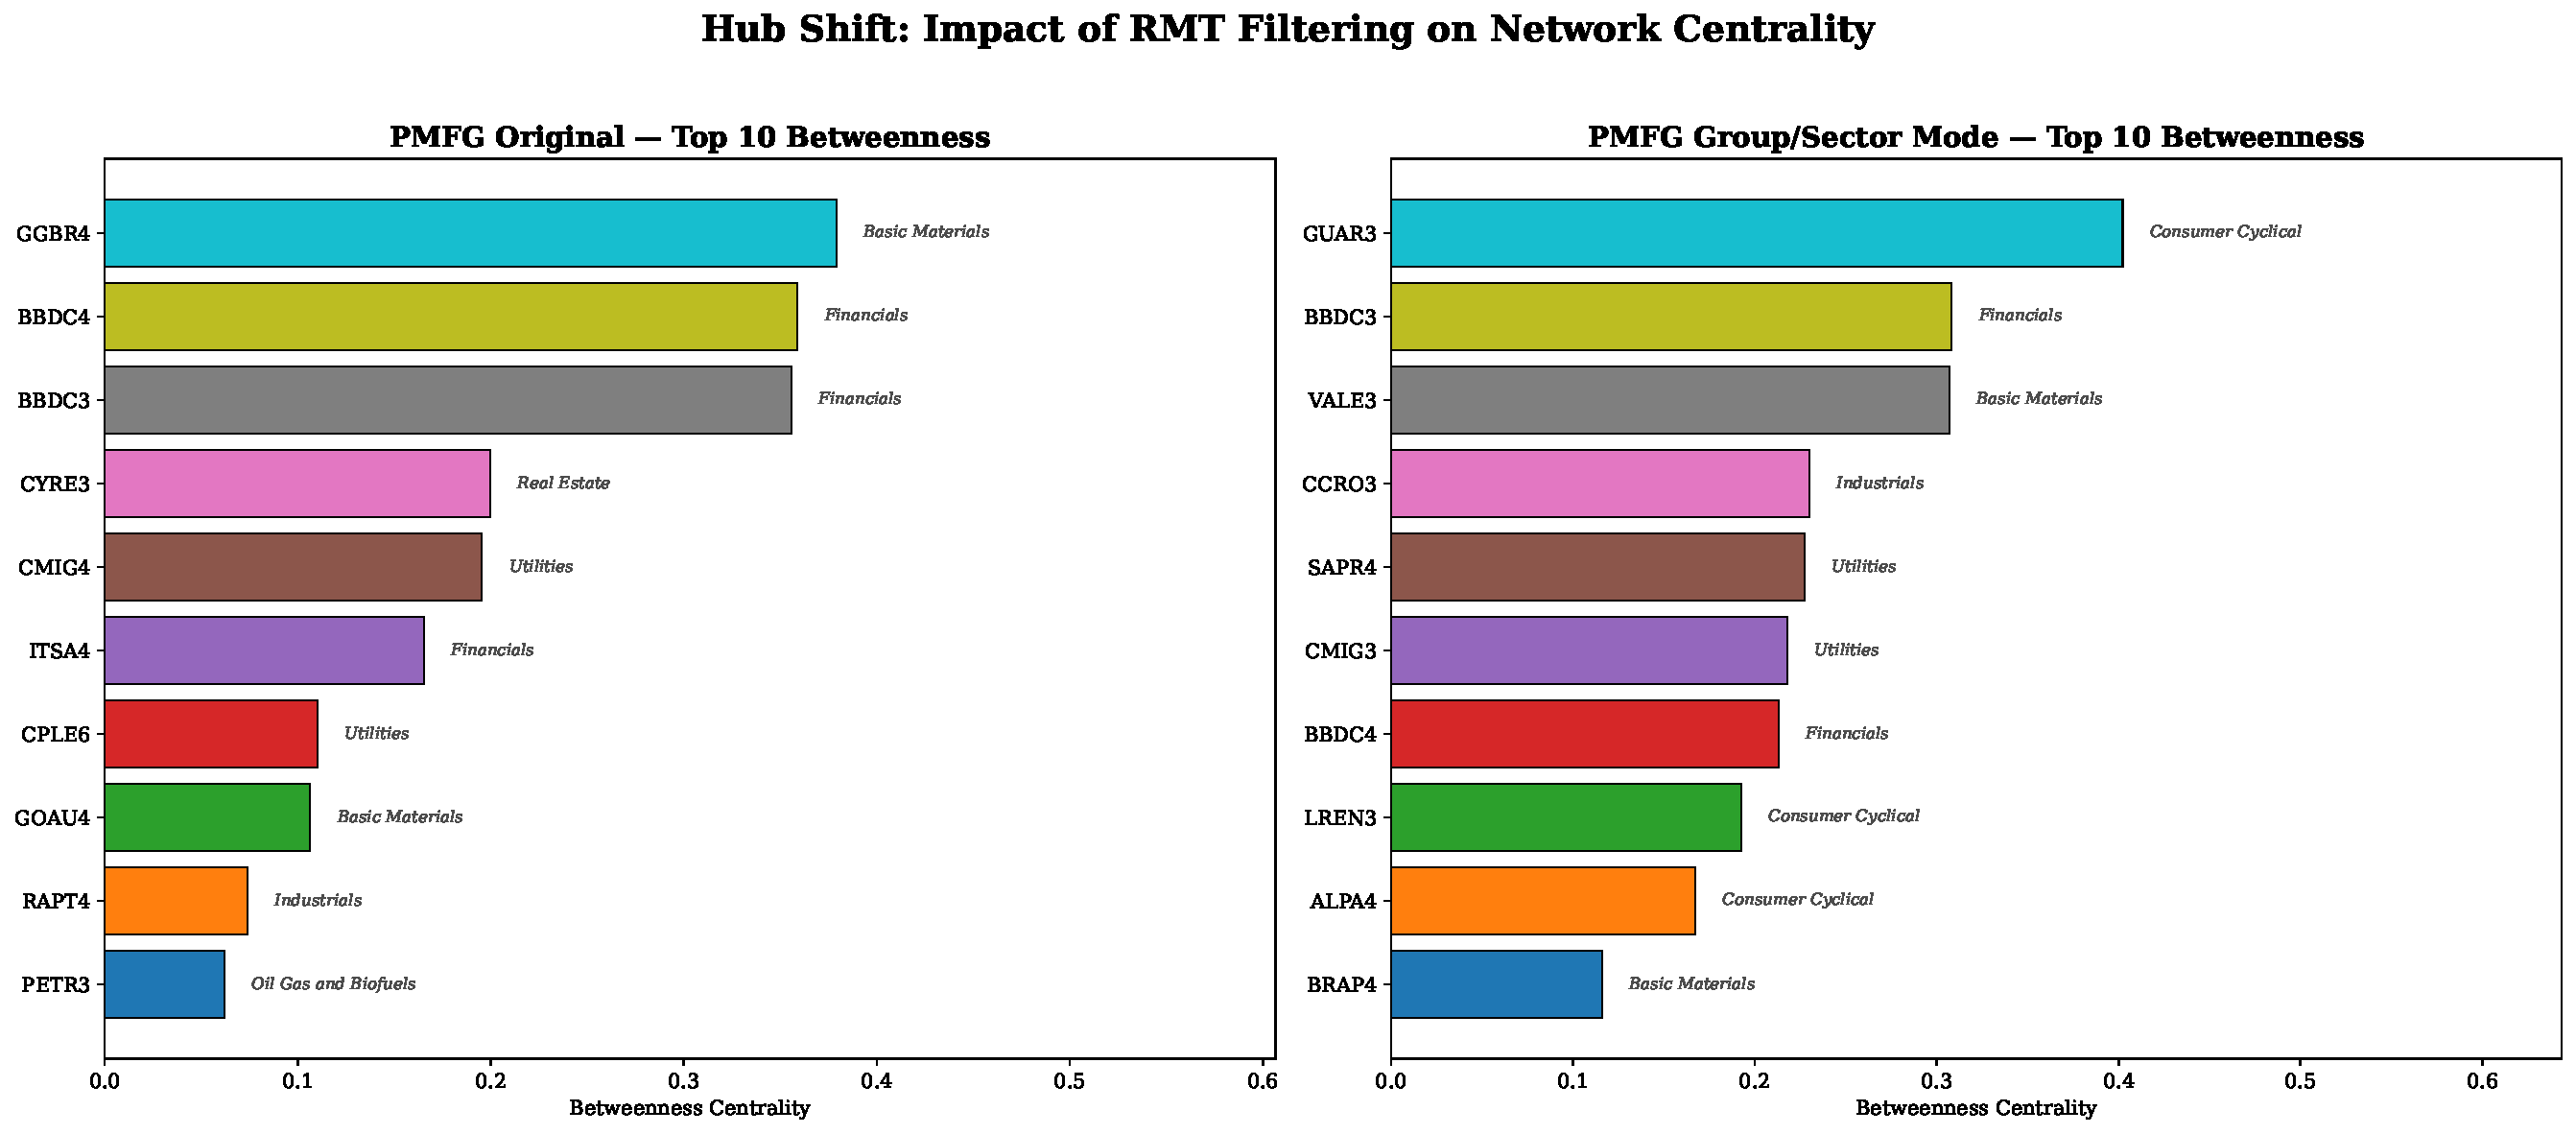
\includegraphics[
width=\linewidth,
height=0.58\textheight,
keepaspectratio
]{images/figure_14_network_hub_rank_comparison.pdf}
\captionof{figure}{Hub-rank comparison across original and group-mode networks. Removal of the dominant market component changes which assets occupy central positions in the dependency structure.}
\label{fig:hub_rank}
\end{center}



\begin{center}
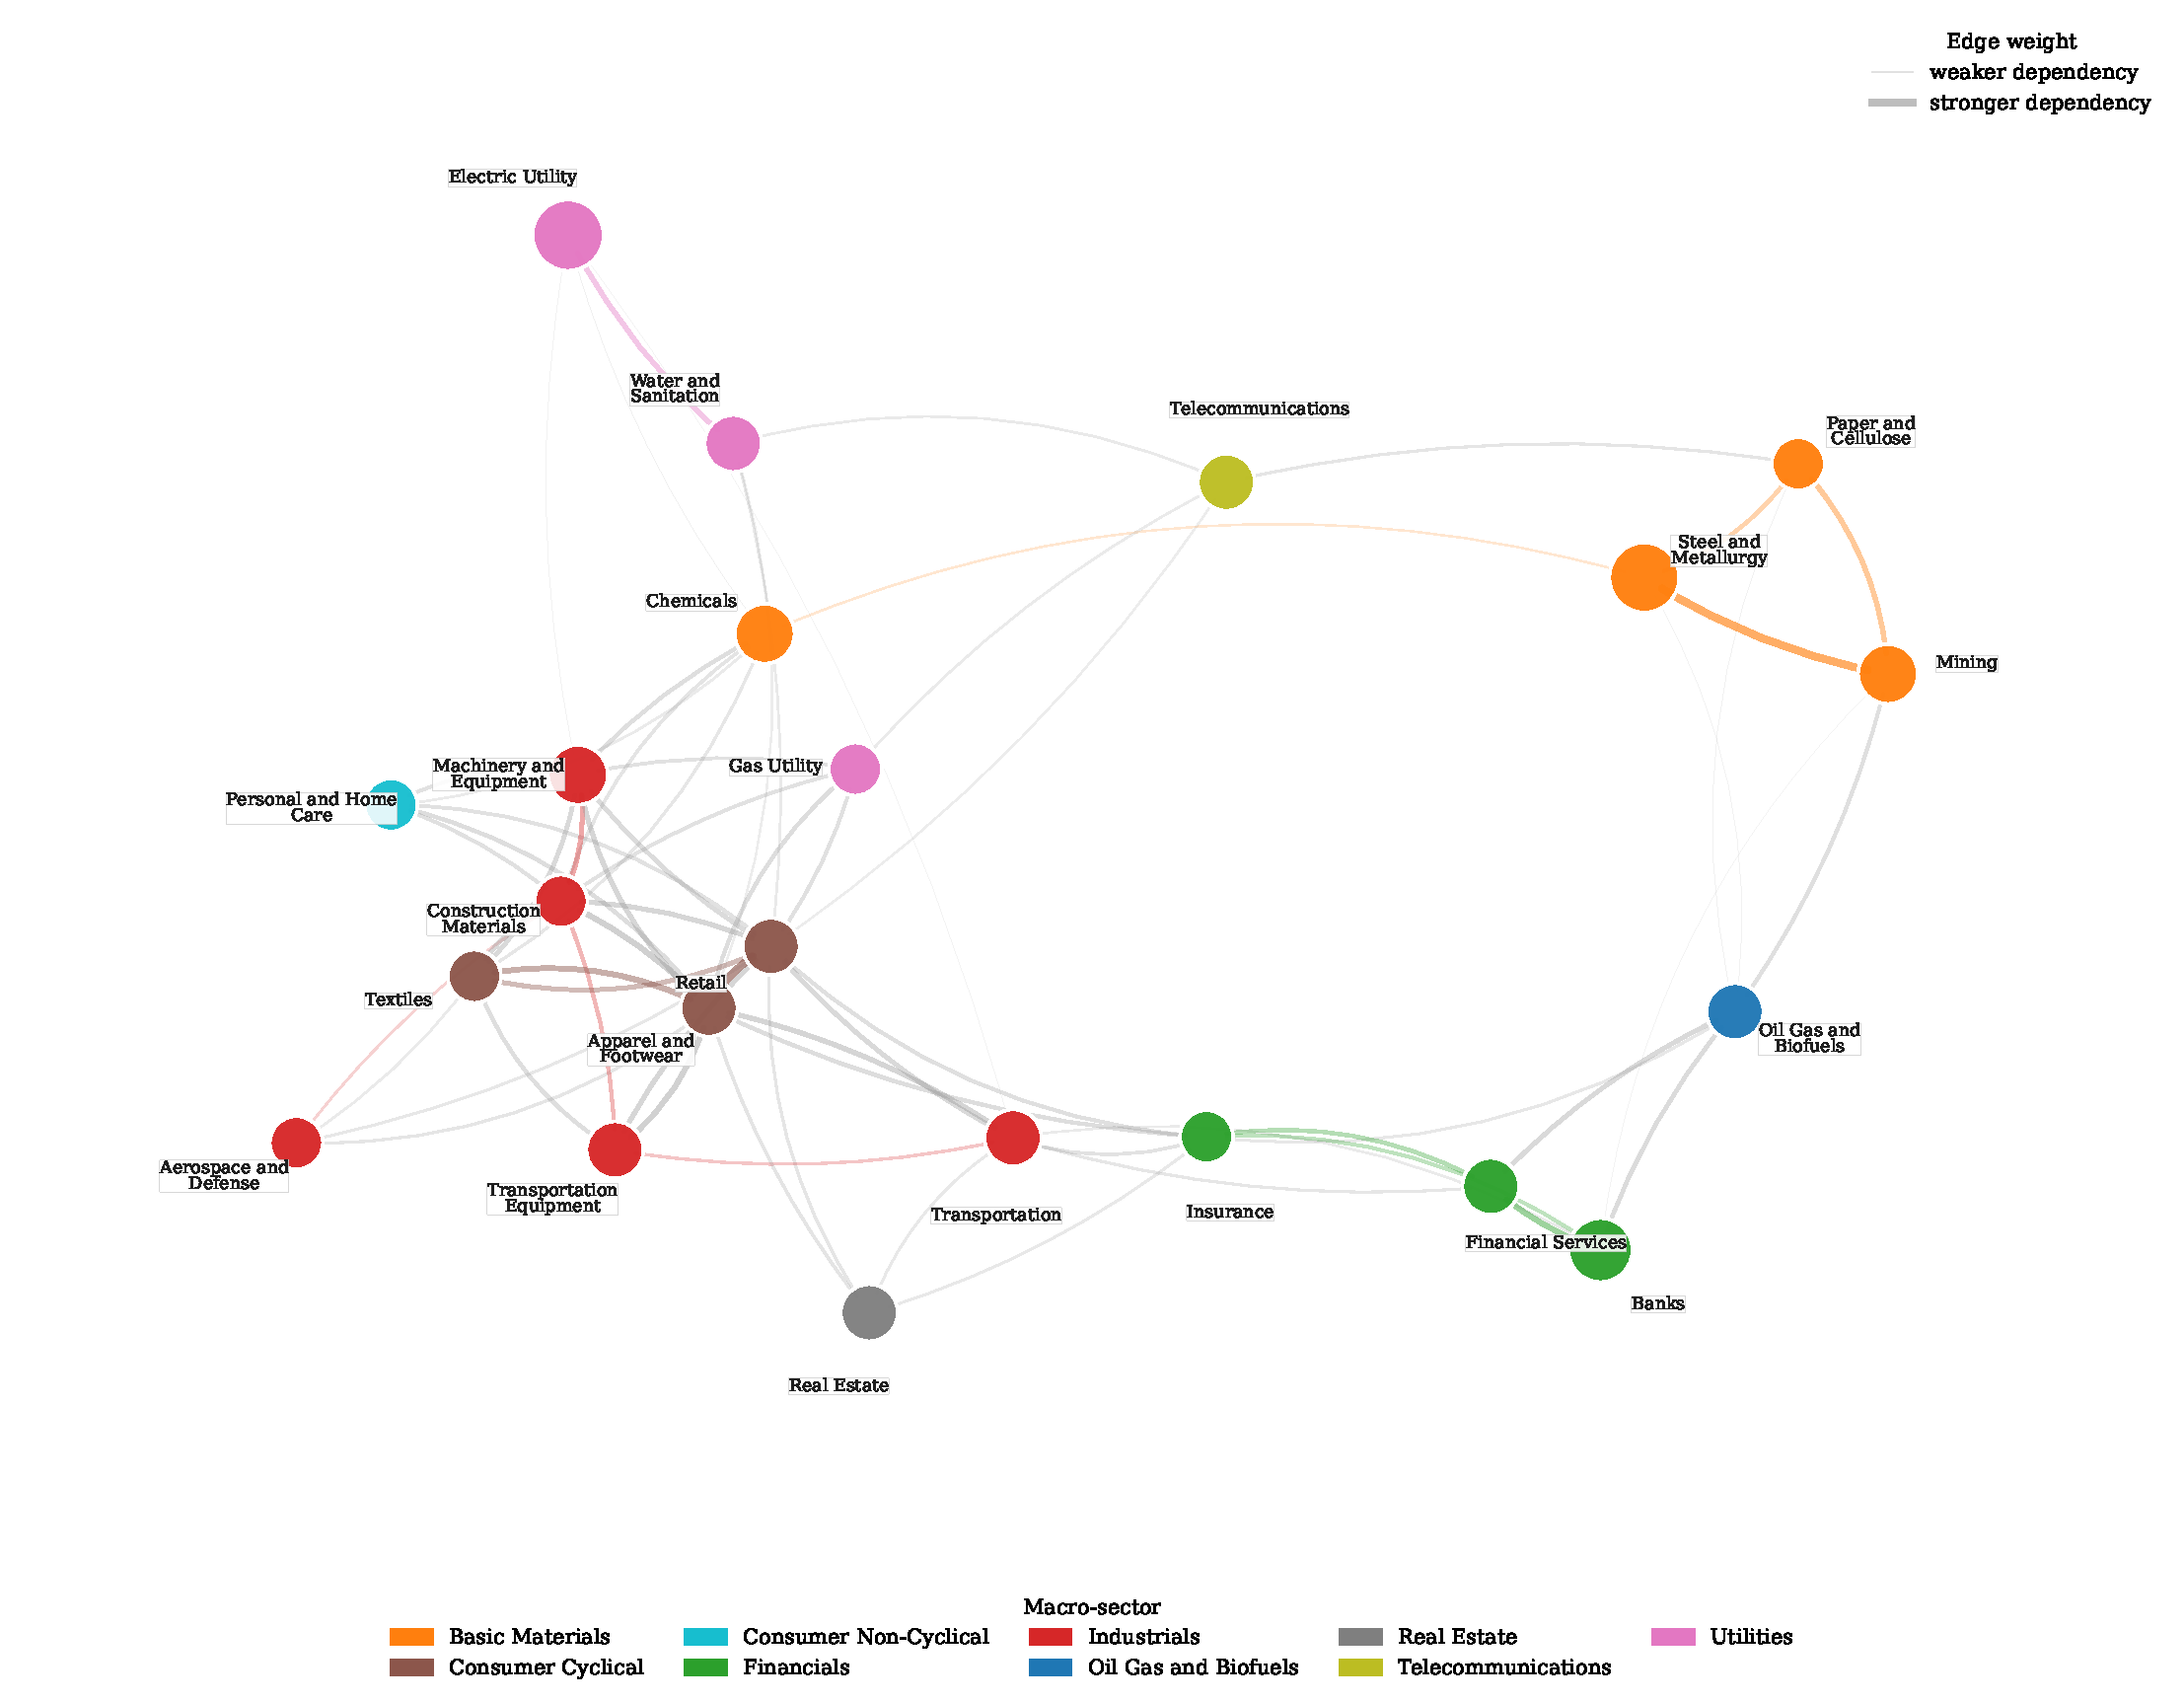
\includegraphics[
width=0.92\linewidth,
height=0.58\textheight,
keepaspectratio
]{images/figure_15_subsector_dependency_network.pdf}
\captionof{figure}{Aggregated subsector dependency network. Nodes represent subsectors, node colour identifies the macro-sector and node size is proportional to the number of assets in each subsector. Edge thickness represents the average retained dependency between connected subsectors.}
\label{fig:subsector_network}
\end{center}

The original-network hubs can reflect both localized relationships and exposure to the broad common component. After market-mode removal, the central nodes instead characterize the residual dependency structure. Assets such as GUAR3, BBDC3, VALE3, CCRO3, SAPR4 and CMIG3 consequently gain prominence in the group-mode rankings. These rankings are interpreted as descriptive full-sample configurations rather than permanent structural labels, since their temporal stability is examined separately in Section~\ref{sec:robustness}.

To translate this ticker-level organization into a more interpretable economic representation, we aggregate the retained dependencies by subsector. The resulting network contains 22 subsectors and 66 undirected links, with density 0.2857. Its mean and median edge dependencies are 0.0566 and 0.0561, respectively. These relatively small values are expected because the graph summarizes dependencies after spectral filtering and aggregation rather than raw pairwise correlations.

Figure~\ref{fig:subsector_network} shows the resulting subsector-level structure. Nodes represent subsectors, node colours indicate macro-sectors, and node sizes reflect the number of constituent assets. Edge thickness represents the average retained dependency between the corresponding subsectors.

The aggregated network reveals different forms of structural importance. Retail has the highest degree, indicating the largest number of retained direct subsector connections. Electric Utility has the highest betweenness, placing it in a bridge-like position between different parts of the graph. Apparel and Footwear has the highest weighted degree, indicating that its retained connections are comparatively strong. These differences show that connectivity, bridging position, and dependency intensity capture distinct aspects of the residual market structure.

The subsector representation therefore provides an economic summary of the organization identified previously at the spectral and ticker-network levels. The analysis begins with non-leading RMT modes, shows that localized structure persists in hierarchical and graph representations, and finally translates the retained network relationships into sectoral and subsector-level organization. This completes the structural part of the empirical analysis before the robustness tests and retrospective volatility-model assessment.
